\documentclass{article}

\usepackage{graphicx}
\usepackage{subcaption}

\begin{document}

\begin{figure}
    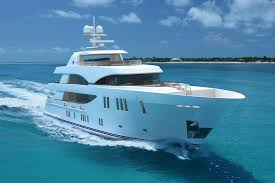
\includegraphics[width=\linewidth]{boat.jpg}
    \caption{A boat.}
    \label{fig:boat1}
\end{figure}

Figure \ref{fig:boat1} shows a boat.

\begin{figure}[h!]
    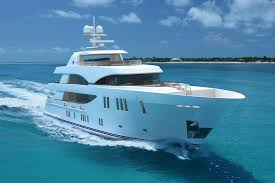
\includegraphics[width=\linewidth]{boat.jpg}
    \caption{A boat (float).}
    \label{fig:boat2}
\end{figure}

\begin{figure}[h!]
    \centering
    \begin{subfigure}[b]{0.4\linewidth}
        
\includegraphics[width=\linewidth]{coffee.jpg}
        \caption{Coffee.}
    \end{subfigure}
    \begin{subfigure}[b]{0.4\linewidth}
        
\includegraphics[width=\linewidth]{coffee.jpg}
        \caption{More coffee.}
    \end{subfigure}
    \caption{The same cup of coffee. Two times.}
    \label{fig:coffee}
\end{figure}

\begin{figure}[h!]
    \centering
    \begin{subfigure}[b]{0.2\linewidth}
        
\includegraphics[width=\linewidth]{coffee.jpg}
        \caption{Coffee.}
    \end{subfigure}
    \begin{subfigure}[b]{0.2\linewidth}
        
\includegraphics[width=\linewidth]{coffee.jpg}
        \caption{More coffee.}
    \end{subfigure}
    \begin{subfigure}[b]{0.2\linewidth}
        
\includegraphics[width=\linewidth]{coffee.jpg}
        \caption{Tasty coffee.}
    \end{subfigure}
    \begin{subfigure}[b]{0.5\linewidth}
        
\includegraphics[width=\linewidth]{coffee.jpg}
        \caption{Too much coffee.}
    \end{subfigure}
    \caption{The same cup of coffee. Multiple times.}
    \label{fig:coffee3}
\end{figure}

\end{document}
